\documentclass[titlepage]{article}

\usepackage{amsmath}
\usepackage{hyperref}
\usepackage{graphicx}
\graphicspath{ {./imgs/} }

\begin{document}

\title{
    PHYS 350 Final Project \\
    \large Bobbing in Air
}
\author{Axel Jacobsen \\ 21341169}
\maketitle

\tableofcontents
\newpage

\section{The Question}

I thought of this idea for a project while on a run. I was thinking about the forces and energy of an object bobbing in water, and was trying to think of other examples of the same motion in nature. From there, I tried to imagine some object bobbing in air. Then I thought of blimps and hot air balloons! Since they are just buoyant objects in their own (albiet low-density) fluid, I wanted to figure out if blimps would ``bob'' in the atmosphere as it reaches its max altitude.

\section{The Model}

Lighter-than-air aircraft (LTAA) are remarkably simple. In the simplest cases, one can model a LTAA as a volume, with some point mass in the center. We need some non-zero volume for the buoyant force. More complex models can model some massles volume connected to a mass by a massless rigid body, as shown below:

\begin{figure}[h]
    \centering
    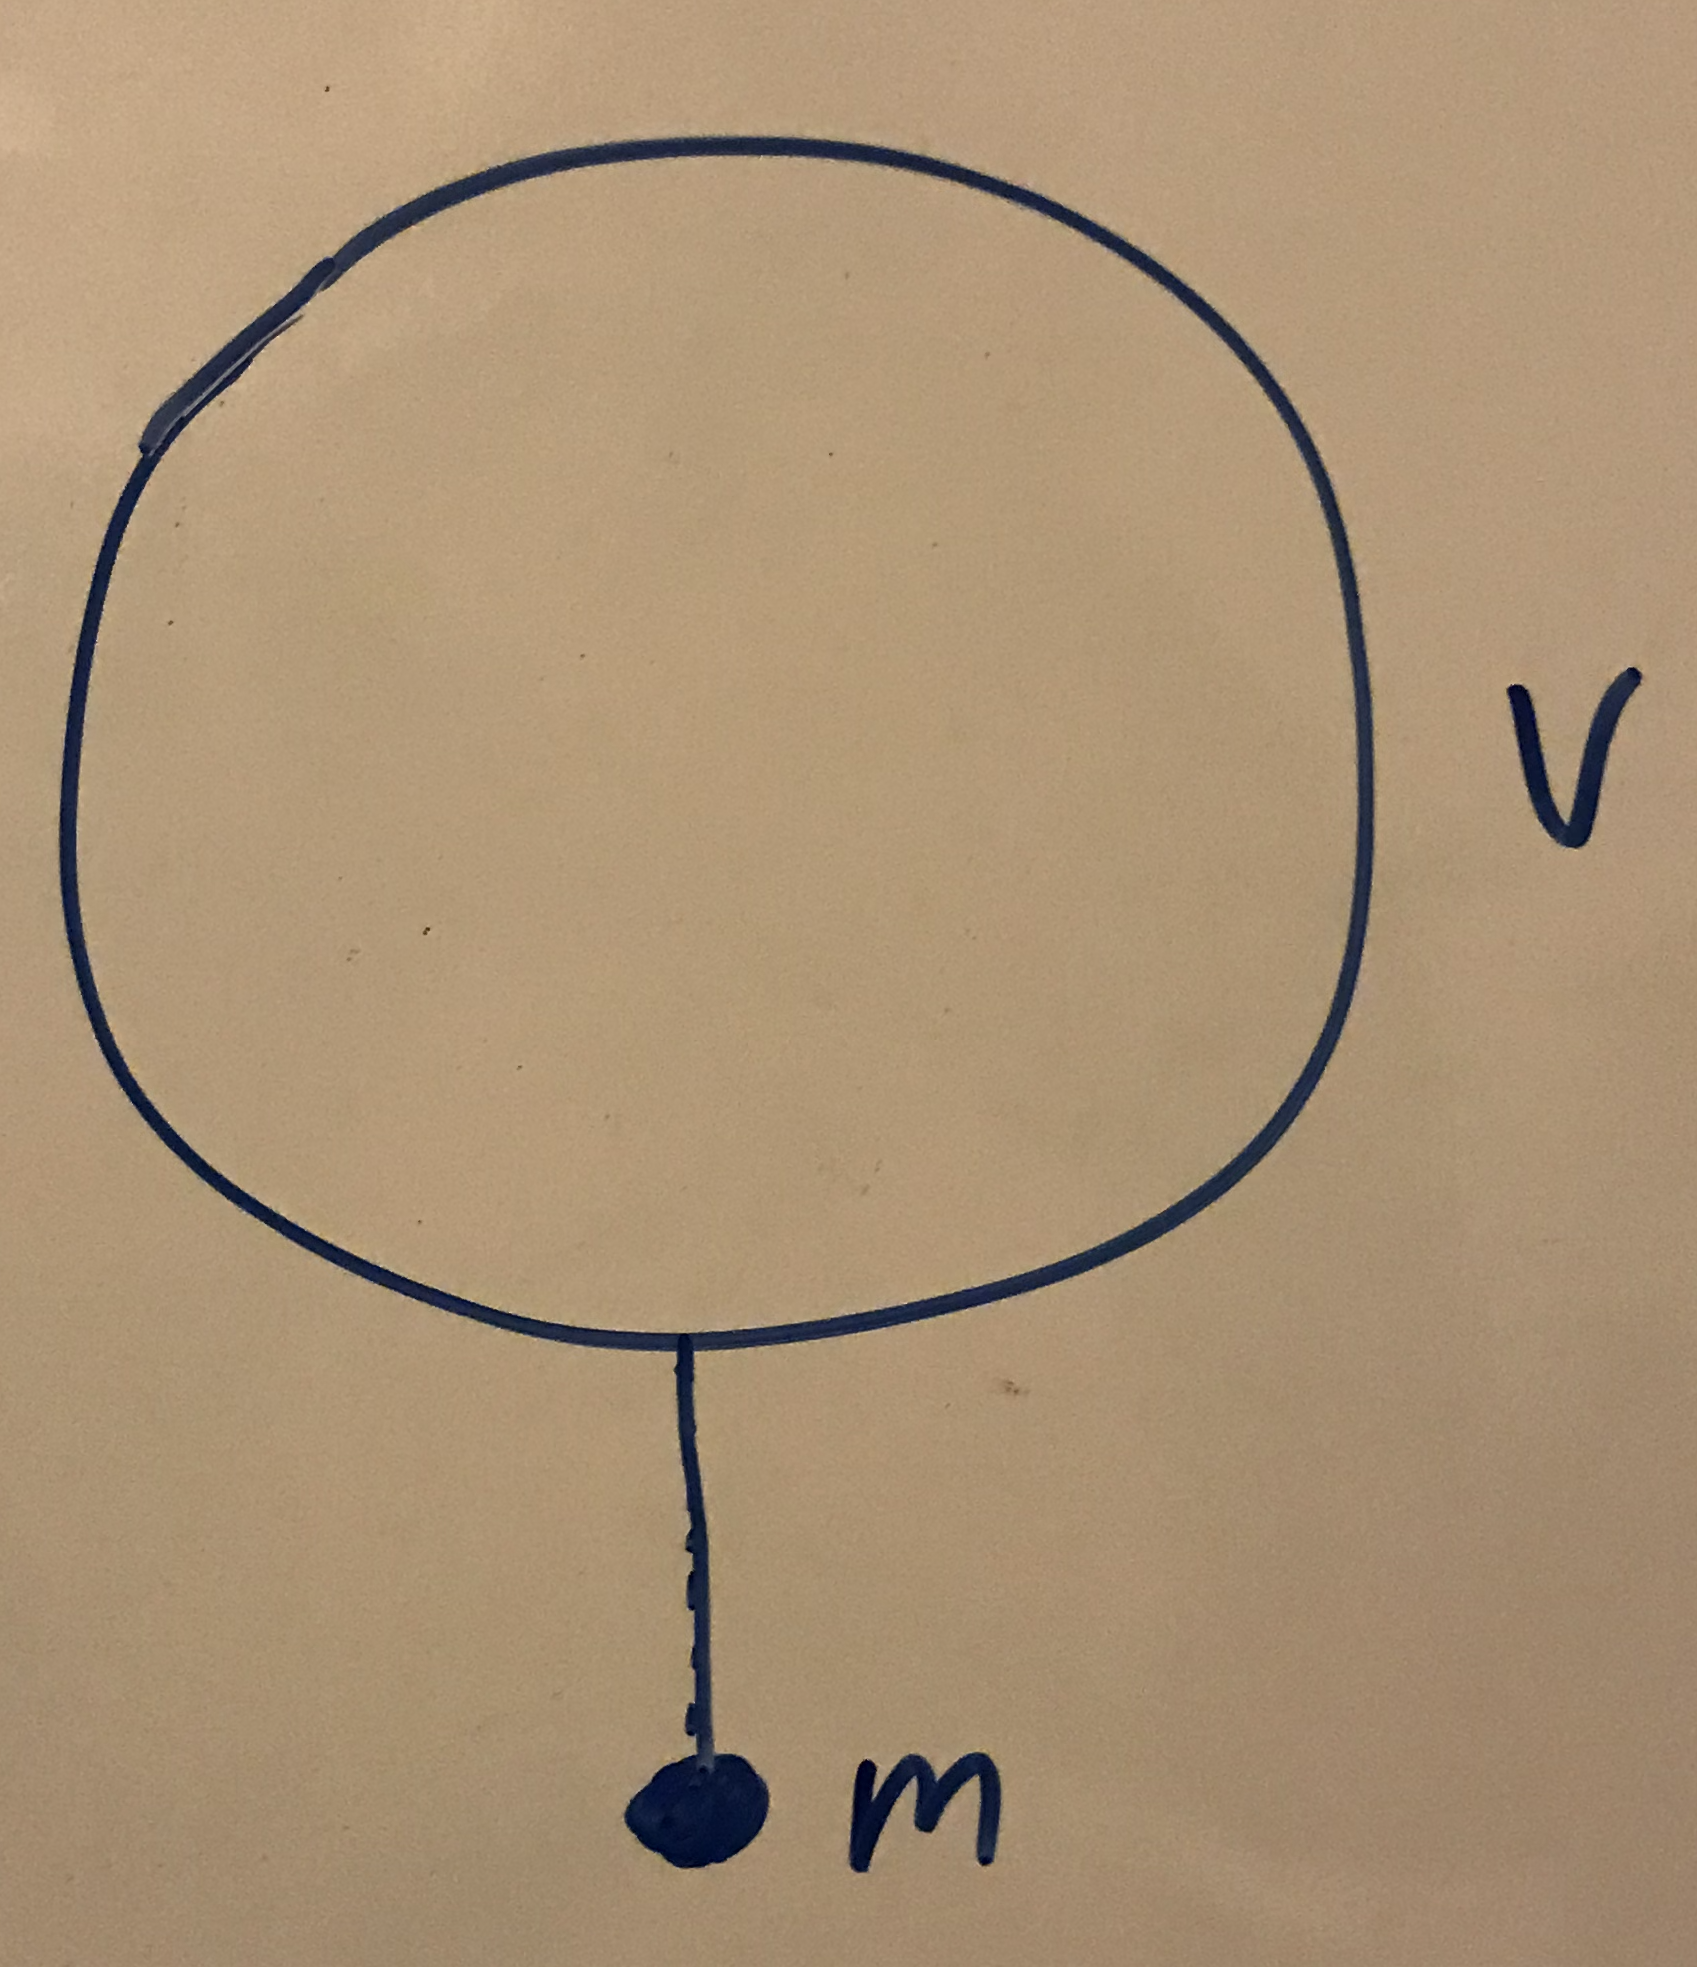
\includegraphics[width=100px]{balloon.png}
    \caption{Balloon Model}
\end{figure}

This would allow for more dimensions of motion; for example, you could tilt the balloon a little bit and you would get oscillations back and fourth:

\begin{figure}[h]
    \centering
    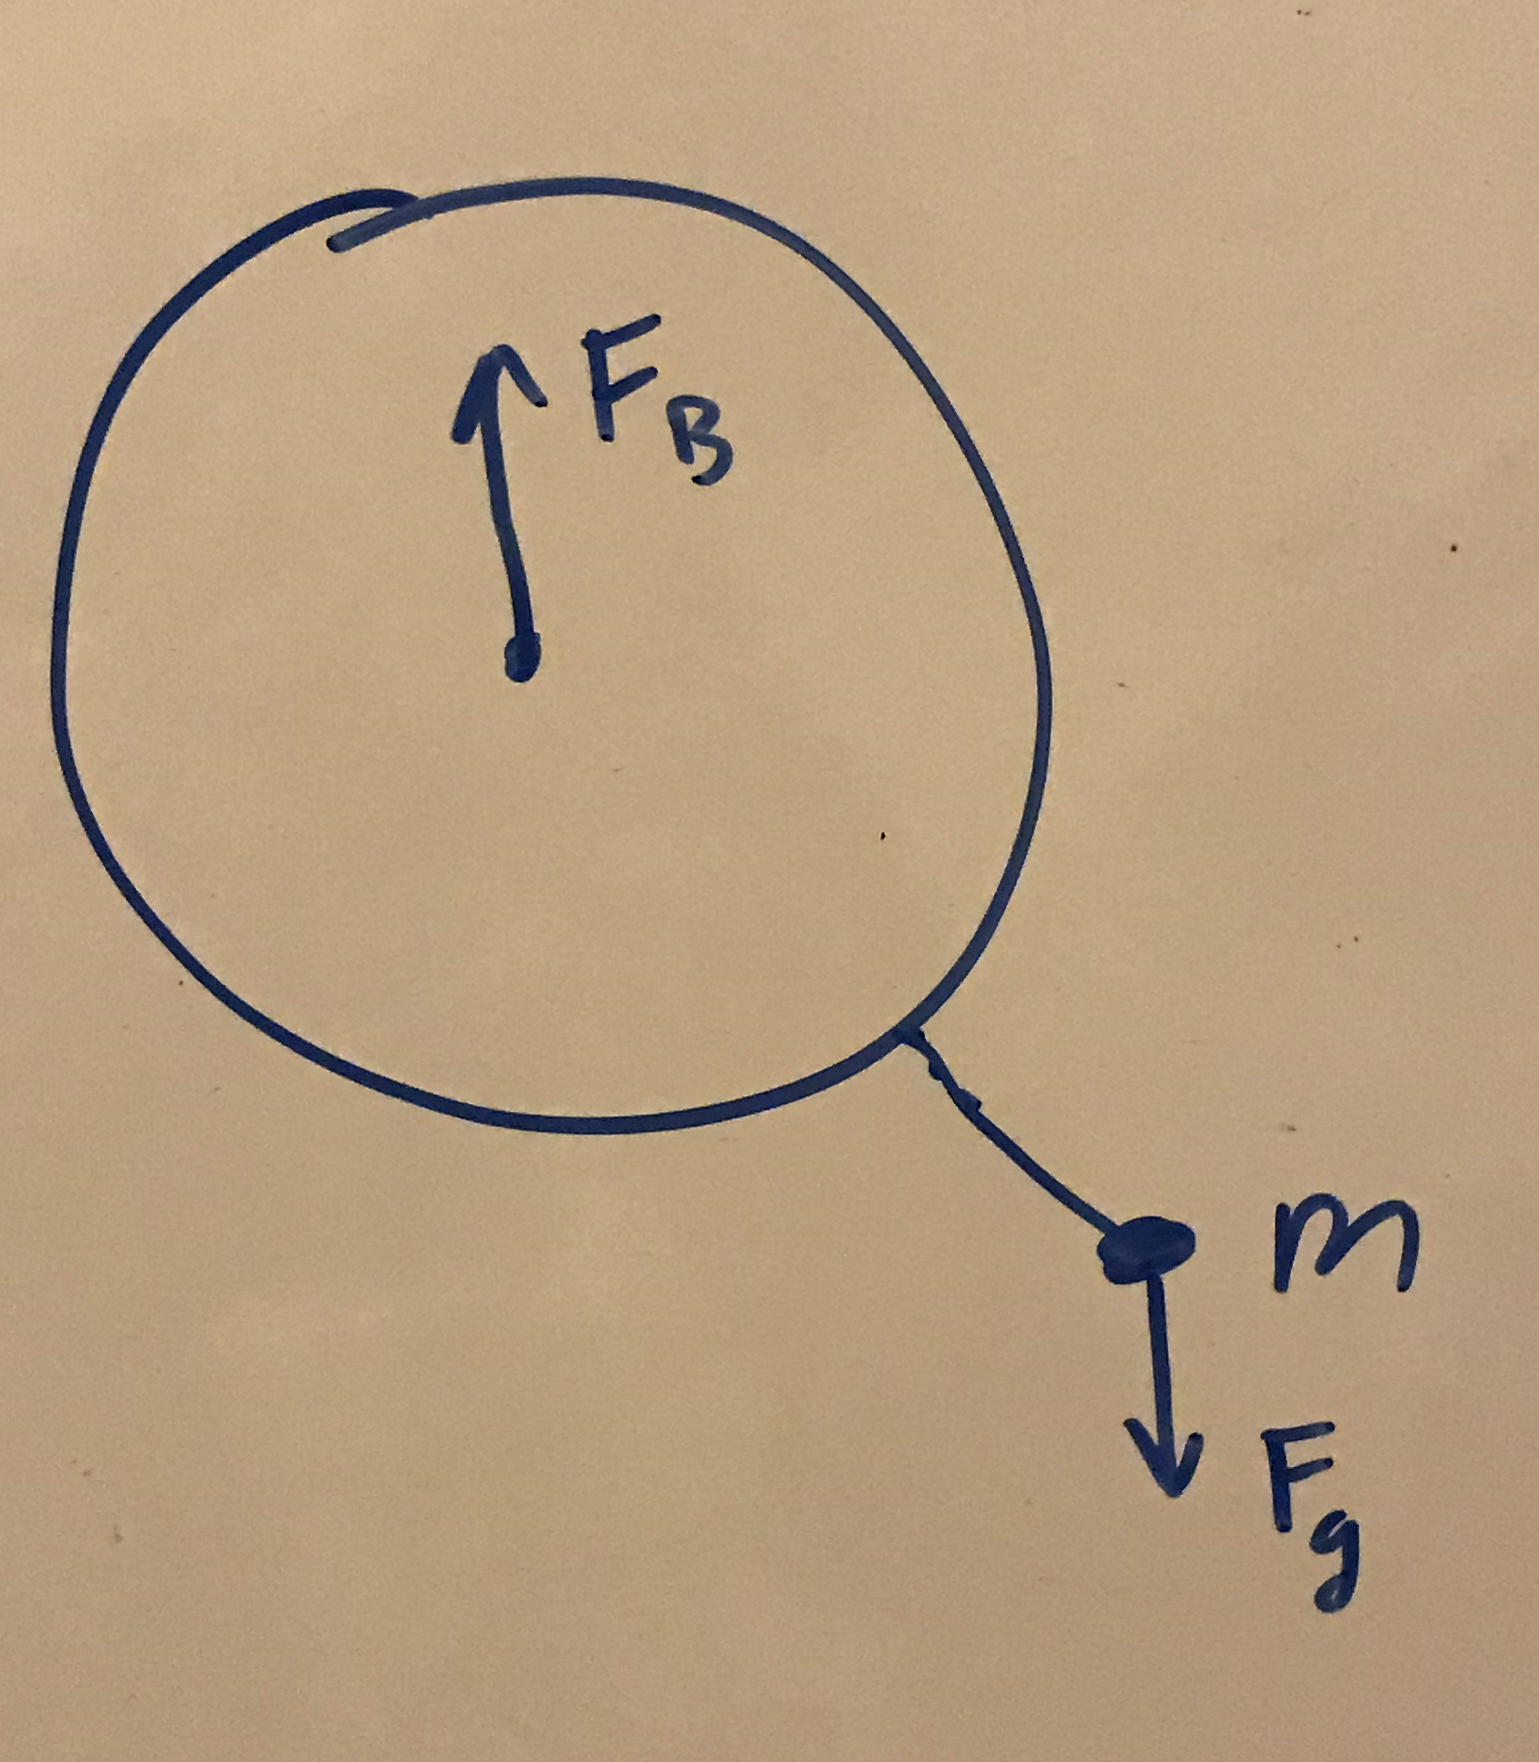
\includegraphics[width=100px]{balloon_angle.png}
    \caption{Balloon Model, perturbed by some angle}
\end{figure}

However, we should stay on track (for now). We have to contend with a model for the atmosphere. We need the "buoyant potential" for this probem, and for that, we need the air density. Gasses are nothing if not unruly, with their properties of pressure, temperature, and density being interconnected. This is, of course, assuming that the atmosphere is an ideal gas, which it is not (due to the presence of water vapor). Lucky for me, we have an expression for density over altitude. Wikipedia's page on the Density of Air\cite{density_eqn} gives us

\[
    \rho=\frac{p_{0} M}{R T_{0}}\left(1-\frac{L z}{T_{0}}\right)^{g M / R L-1}
\]

where

\[
     \begin{split}
        &\rho \rightarrow \text{Air Density} \\
        &p_0 \rightarrow \text{Air Pressure at Sea Level} \\
        &M \rightarrow \text{Molar Mass of Air} \\
        &R \rightarrow \text{Ideal Gas Constant} \\
        &L \rightarrow \text{Temperature Lapse Rate} \\
        &T_0 \rightarrow \text{Temperature at Sea Level} \\
        &g \rightarrow \text{Gravitational Acceleration Near Earth} \\
    \end{split}
\]

This equation was derived assuming only that air is an ideal gas. If we make the assumption that air is isothermal (which is not a terrible approximation within the Troposphere \cite{troposphere}, which extends to ~12 km), we can use the further simplification of

\[
    \rho(z) \approx \rho_{0} e^{-z / H_{n}}
\]

where $H_n$ is approximately $10.4~km$, and $\rho_0$ is the density of air at sea level.

With $ \rho_0 = 1.225 kg/m^3 $\cite{density_eqn} , we can proceed to the problems!

\section{Problems}

\subsection{Problem 1: What is the altitude over time of a unperturbed blimp?}

Imagine a blimp of volume $V$ and mass $m$, initially stationary, fixed to the ground. If the air has a density of $\rho(z) = \rho_0 e^{-{z / H}} $, what is its motion over time? Assume that it is constrained to only move vertically. You can solve it numerically.

\subsection{Problem 2: Adding air resistance}

A fault of the previous question is that we ignore air resistance. However, integrating air resistance into the Lagrangian is not a straitforward task, as air drag is a \textit{dissipative} force. The Euler-Lagrange Equations only hold for conservative forces, where energy is conserved. However, Lord Raleigh suggested \cite{raleigh} that a dissipative force $D$ could be added if it had the form 
\[
    D=\frac{1}{2} \sum_{j=1}^{m} \sum_{k=1}^{m} C_{j k} \dot{q}_{j} \dot{q}_{k} 
\]
where the sums are over all of the generalized coordinates. The Euler-Lagrange equation would be modified to
\[
    \frac{\mathrm{d}}{\mathrm{d} t}\left(\frac{\partial L}{\partial \dot{q}_{j}}\right)-\frac{\partial L}{\partial q_{j}}+\frac{\partial D}{\partial \dot{q}_{j}} = 0 
\]
Luckily, air drag has a formula which fits Lord Raleigh's dissipative force \cite{drag}
\[
    F_{D}=\frac{1}{2} \rho v^{2} C_{D} A 
\]
where $v$ is relative velocity to the air, $C_D$ is the coefficient of drag, and $A$ is the incident area of the object. This has the form of $D$, as 
\[
    \begin{split}
        C_{jk} = \rho C_D A \\
        \sum_{j=1}^{m} \sum_{k=1}^{m} \dot{q}_{j} \dot{q}_{k} = \dot {z}^2
    \end{split}
\]
With this, find the blimps motion over time. You can solve it numerically.


\newpage

\section{Solutions}

\subsection{Solution: Problem 1}

This is an $s = 1$ problem, with $q = z$. We fix the origin of the system to the ground, with $z$ pointing vertically. We need to figure out the ``potential'' for the buoyant force. Remembering that
\[
    \textbf{F} = - {\partial U \over \partial r} \hat{r},
\]
we can find the potential from the buoyant force. The equation for the buoyant force is
\[
    \begin{split}
        \textbf{F}_b &= - \rho(z) V \textbf{g} \\
        &= - \rho_{0} e^{-z / H_{n}} V \textbf{g} \\
    \end{split}
\]
so
\[
    \begin{split}
        U_b &= - \int_0^z \textbf{F} \cdot d\textbf{r} \\
        &= \int_0^z \rho_{0} e^{-r / H_{n}} V \textbf{g} \cdot d\textbf{r} \\
        &= H_n \rho_0 e^{-z/H_n} V g
    \end{split}
\]
The sign of $U_b$ is positive as the integral of $e^{-x}$ is negative, and $\textbf{g} \cdot d\textbf{r} = -g dr$. We have the gravitational potential $U_g = mgz$. The kinetic energy of the blimp is $T = {m \over 2} \dot{z}^2$. The Lagrangian then must be
\[
    \begin{split}
        \mathcal{L} &= T - U \\
        &= {m \over 2} \dot{z}^2 - H_n \rho_0 e^{-z/H_n} V g - mgz
    \end{split}
\]
Applying the Euler-Lagrange equation,
\[
    {d \over dt} \left( m\dot{z} \right) = \rho_0 e^{-z / H_n} V g - mg
\]
so our equation of motion is
\[
    m\ddot{z} - \rho_0 e^{-z / H_n} V g + mg = 0
\]
This is a non-linear, non-homogenous, 2nd order ordinary differential equation. Therefore, we will sove this numerically. We can do this by letting $v = \dot{z}$, and solving the following system of equations. 
\[
    \begin{cases}
        \dot{z} = v \\
        \dot{v} = \ddot{z} = {\rho_0 \over m} e^{-z / H_n} V g - g
    \end{cases}
\]

\newpage

We will have to assign numerical values for the volume and the mass of the ship; we can use the mass and volume of a Hindenburg, which had a volume of $V = 200,000~m^3$ and a mass of $474,000~lbs$, or $215,000~kg$ \cite{zeppelin}. With a little python (which is in the appendix), we have a solution for the blimp's altitude over time:
\begin{figure}[h]
    \centering
    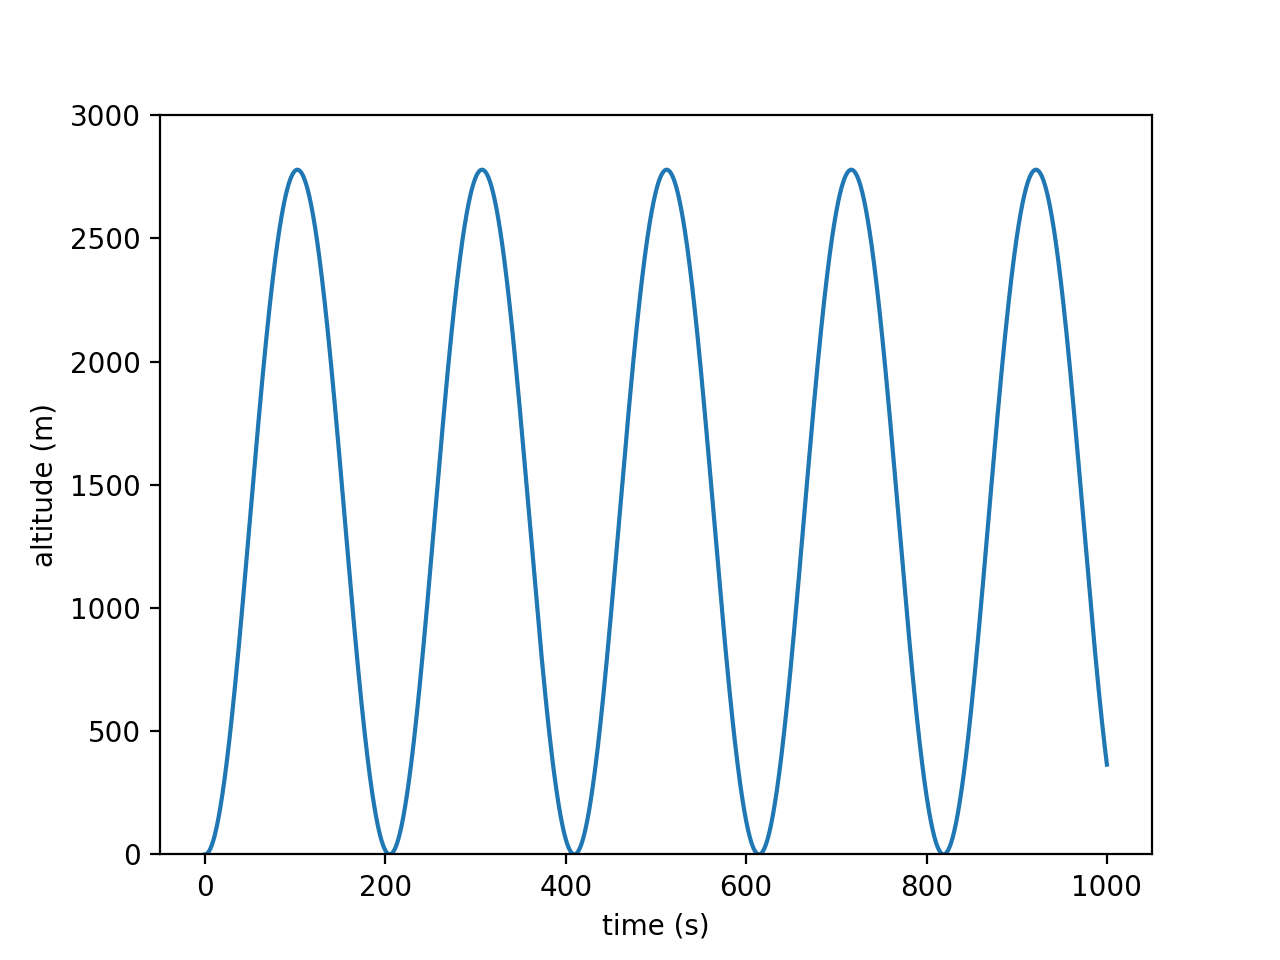
\includegraphics[width=250px]{p1_0m_release.png}
    \caption{Altitude over time of a blimp, released from the ground}
\end{figure}
To my suprise, the solution to the ODE is sinusoidal; The blimp rockets upward to a max altitude of ~$2778~m$, before descending again to tap the Earth, just to rocket up again. This actually makes sense; I ignored air drag, and the lagrangain for this system does not depend on time, so energy is conserved.

\newpage
What if we release the blimp at some altitude greater than 0, say $1000~m$? After changing the initial conditions and numerically solving again, the altitude over time is given by Figure \ref{fig:1000mrelease}.
\begin{figure}[h!]
    \centering
    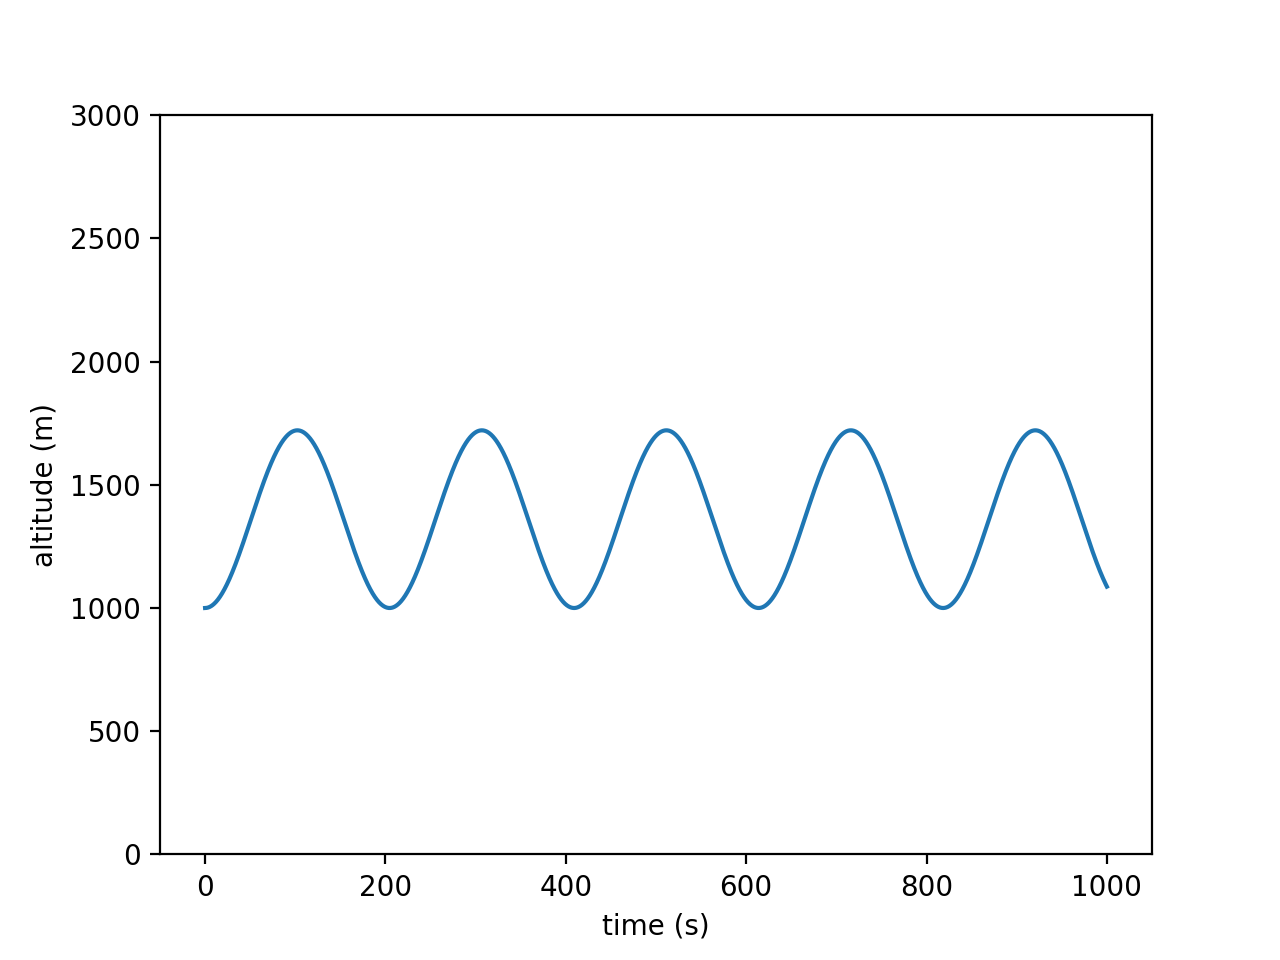
\includegraphics[width=250px]{p1_1000m_release.png}
    \caption{Altitude over time of a blimp, released from 1000 meters in the air}
    \label{fig:1000mrelease}
\end{figure}
And as expected, the blimp oscillates with a minimum altitude of 1000 meters. The blimp's maximum height is also proportionally lower, which makes sense, as the buoyant potential energy decreases exponentially, where the gravitational potential energy only increases linearly.
\vspace{8pt}

While this is neat, it is not very realistic. For one, I am completely neglecting air resistance, which would have a large factor for the blimp's position over time, especially with it's high speeds. The next question will go a little bit into trying to integrate a dissipative force into Lagrangian Mechanics.

\subsection{Solution: Problem 2}

We are given the formula for air drag - before we can use it, we need to find $C_D$ and $A$. Lets use a Zeppelin again. For the $C_D$, we can use the coefficient of drag of $C_D = 0.023$ \cite{usslosangeles} for the U.S.S. Los Angeles. It is approximately the same size as the Hindenburg aircraft, and in fact it was manufactured by Zeppelin, the same company that make the Hindenberg Aircraft. For area, lets assume that the airship does not rotate, and remains horizontal during its entire flight. The area can be approximated by the area of an ellipse with a minor axis of length of $41.2~m$ and a major length of $247~m$ (i.e. the dimensions of the Hindenberg \cite{zeppelin}). This gives
\[
    A = \pi a b = \pi (41.2~m)(247~m) = 31970~m^2
\]
We can now proceed to answering the question! We can use the same Lagrangian as in the previous question:
\[
    \mathcal{L} = {m \over 2} \dot{z}^2 - H_n \rho_0 e^{-z/H_n} V g - mgz
\]
Applying the Euler-Lagrange Equations with Lord Raleigh's contribution,
\[
    \begin{split}
        {d \over dt} \left( m\dot{z} \right) &= \rho_0 e^{-z / H_n} V g - mg - \frac{\partial}{\partial \dot{z}} \left( \frac{1}{2} \rho_0 \dot{z}^{2} C_{D} A \right) \\
        m\ddot{z} &= \rho_0 e^{-z / H_n} V g - mg -  \rho_0 \dot{z} C_{D} A
    \end{split}
\]
We can reduce this to a set of coupled 1st order equations, like before:
\[
    \begin{cases}
        \dot{z} = v \\
        \dot{v} = \ddot{z} = {\rho_0 \over m} e^{-z / H_n} V g - g - \frac{\rho_0}{m} v C_D A
    \end{cases}
\]
Numerically solving with initial conditions all zero, we get something like this:
\begin{figure}[h]
    \centering
    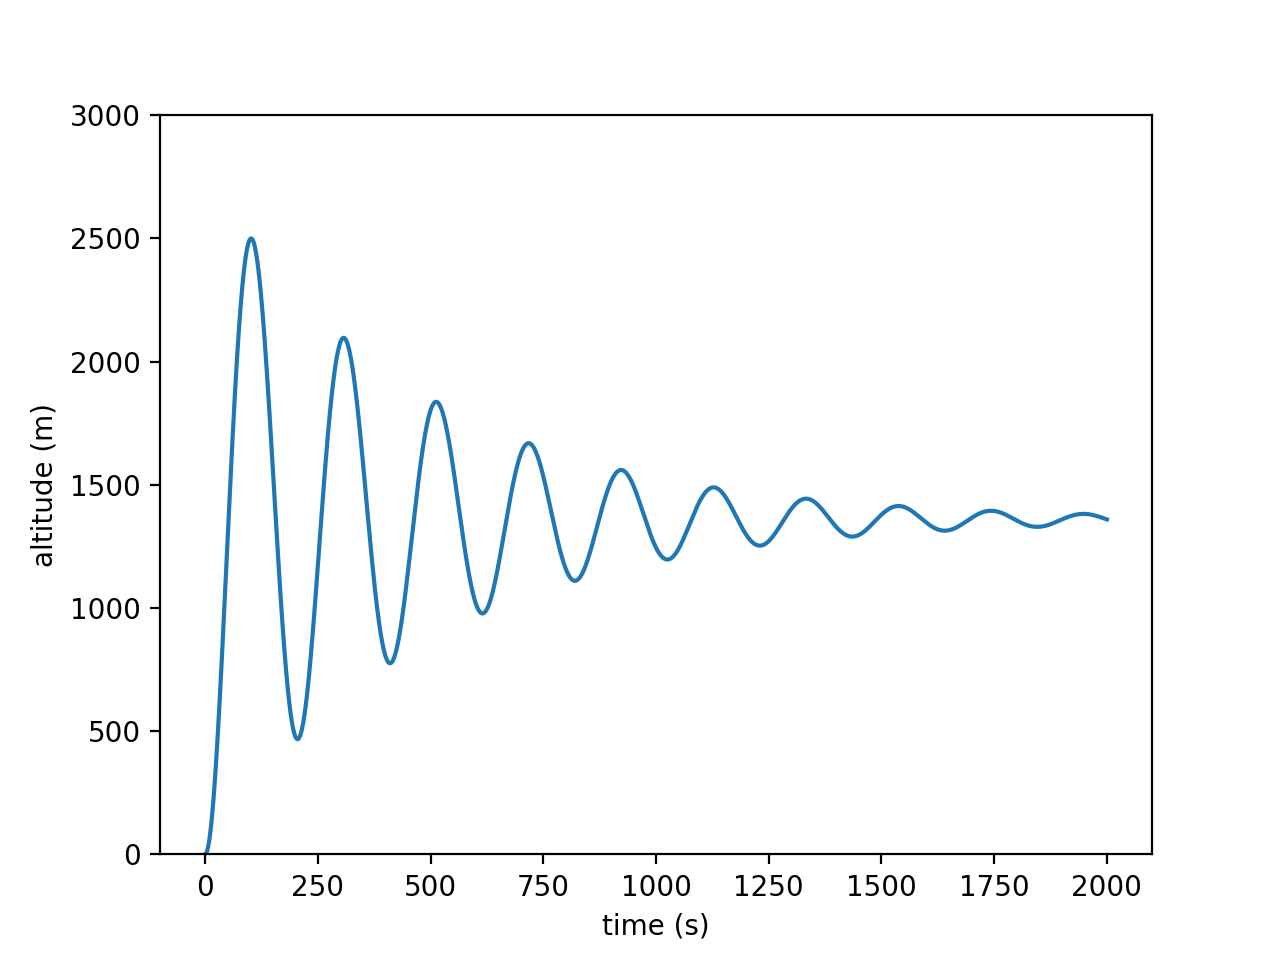
\includegraphics[width=250px]{p2_drag_0.png}
    \caption{The altitude of the blimp over time, starting from the ground}
\end{figure}
This is much nicer! The effect of air drag is clear, as the motion of the blimp is now damped. Releasing from a higher initial altitude, we get
\begin{figure}[h]
    \centering
    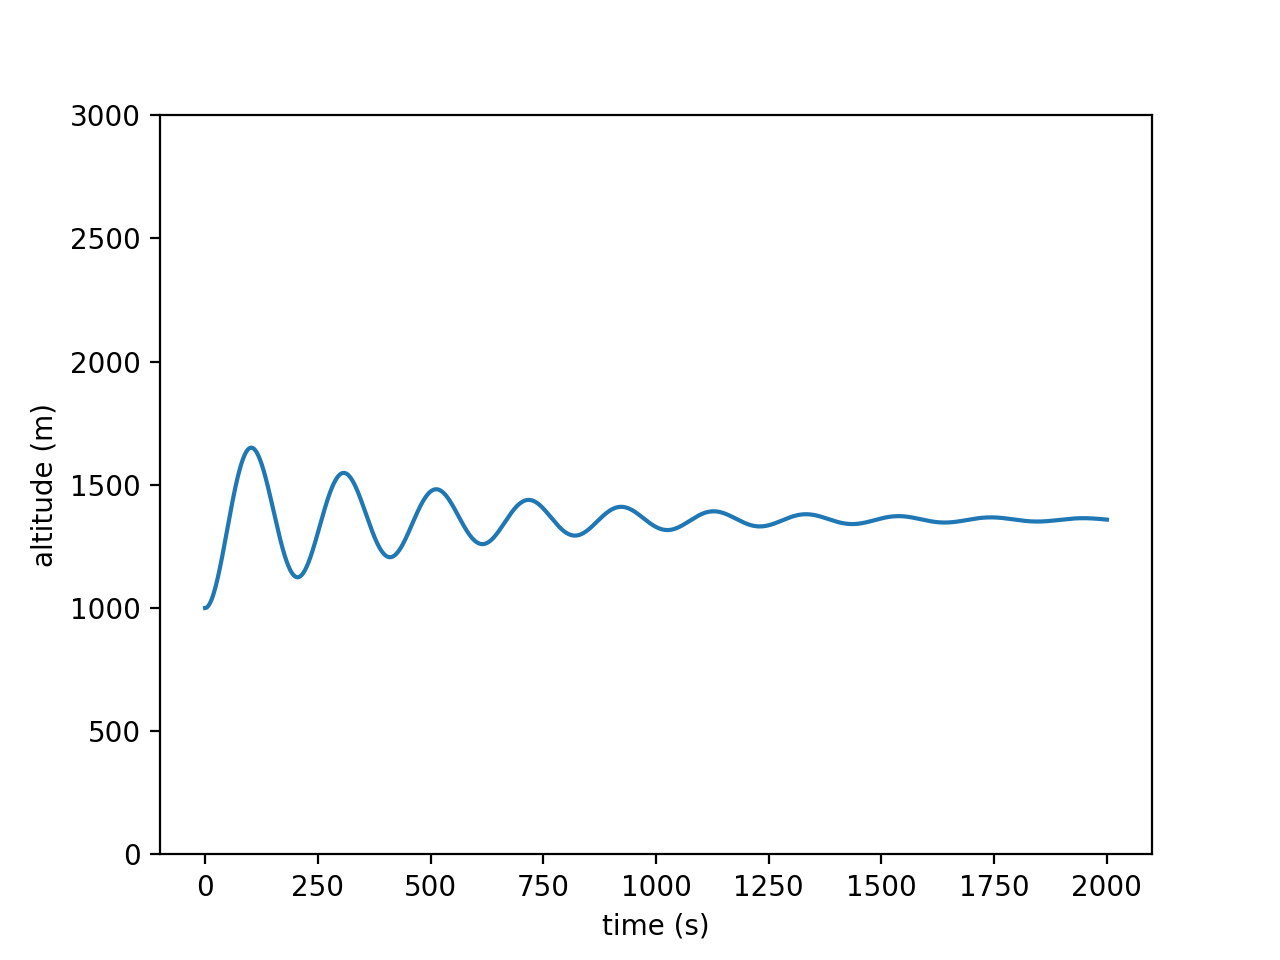
\includegraphics[width=250px]{p2_drag_1000.png}
    \caption{The altitude of the blimp over time, starting 1000 $m$ up}
\end{figure}


\newpage

\bibliographystyle{plain}
\bibliography{references.bib}
\thispagestyle{empty}

\end{document}
